
Conway, by counting the advantage, a player has over the other in a combinatorial game, unveiled a new way to discover numbers. It is clear at this point that numbers are not enough to represent games, but it should in no way discourage anyone interested on them. Until this point, the text showed some instances of the zero and hinted at 1 and -1, and the reader may also know how to build any integer in RB-Hackenbush and Domineering. This chapter shows that knowing that is no more than scratching the surface of surreal numbers.

For the first parts of this section a number \gam{x_1, x_2, ...}{y_1, y_2,...} might be called like a real number: $2, 5, 100000, \frac{1}{3}, \sqrt{10}, \pi$, but there is no reason believe this equality yet. There is also no reason to believe that $1 < 3$ or that 1 + 1 = 2 yet. However, first some numbers will be labeled and only then the proofs are shown.


\subsection*{Finitely Defined Numbers}

It is known that \Gm\ =
\begin{tikzpicture}
	\draw[] (0.3,-0.3) rectangle ++(0.3,0.3);
	\draw[] (0,-0.3) rectangle ++(0.3,0.3);
\end{tikzpicture} = \{ $|$ \{ $|$ \}\} = \{ $|$ 0\} = -1.
What about \Hm\ = 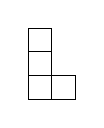
\begin{tikzpicture}
\draw[] (0.3,-0.3) rectangle ++(0.3,0.3);
\draw[] (0,-0.3) rectangle ++(0.3,0.3);
\draw[] (0,0) rectangle ++(0.3,0.3);
\draw[] (0,0.3) rectangle ++(0.3,0.3);
\end{tikzpicture} ?\\


We can find that by calculating G + H + H. To do that, one would usually find the game tree of 
$G + H + H = $
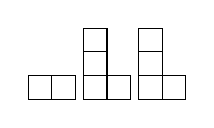
\begin{tikzpicture}
	\draw[] (-0.4,-0.3) rectangle ++(0.3,0.3);
	\draw[] (-0.7,-0.3) rectangle ++(0.3,0.3);
	\draw[] (0.3,-0.3) rectangle ++(0.3,0.3);
	\draw[] (0,-0.3) rectangle ++(0.3,0.3);
	\draw[] (0,0) rectangle ++(0.3,0.3);
	\draw[] (0,0.3) rectangle ++(0.3,0.3);
	\draw[] (1,-0.3) rectangle ++(0.3,0.3);
	\draw[] (0.7,-0.3) rectangle ++(0.3,0.3);
	\draw[] (0.7,0) rectangle ++(0.3,0.3);
	\draw[] (0.7,0.3) rectangle ++(0.3,0.3);
\end{tikzpicture}, and fill the known values bottom-up. However, it is simpler in this case. G + 2H = 0, because whoever starts loses. Since G = 1, H = 1/2. Therefore $H = \{-1, 0 | 1\} = \{0 | 1\} = 1/2$. It might seem weird that a player may be half a move up in a game, if he or she only plays a move, but it is true. It might be valuable to reiterate that H is definitely positive because left wins no matter who starts, but $H < 1$, as left does not have remaining move at the end of the game.

As one gets used to this area of mathematics, it becomes clear that analyzing the game \{1 $|$ \} is the same as analyzing 
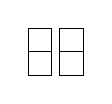
\begin{tikzpicture}
	\draw[] (0.3,-0.3) rectangle ++(0.3,0.3);
	\draw[] (0.3,0) rectangle ++(0.3,0.3);
	\draw[] (-0.1,0) rectangle ++(0.3,0.3);
	\draw[] (-0.1,-0.3) rectangle ++(0.3,0.3);
\end{tikzpicture}, but the former is not reliant on a specific game. Rather, any combinatorial game has an instance equal to \{1 $|$ \}. However, the rules, which have not been presented yet, come from the the mathematical plays. The first practical rule in this text is finding the value of $\{n|\}$ and $\{|{-}n\}$, with n natural.

Of course 
$\underbrace{
	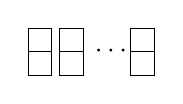
\begin{tikzpicture}
		\draw[] (1.2,-0.3) rectangle ++(0.3,0.3);
		\draw[] (1.2,0) rectangle ++(0.3,0.3);
		\draw[] (-0.1,0) rectangle ++(0.3,0.3);
		\draw[] (-0.1,-0.3) rectangle ++(0.3,0.3);
		\draw[] (0.3,0) rectangle ++(0.3,0.3);
		\draw[] (0.3,-0.3) rectangle ++(0.3,0.3);
		\node at (0.95, 0) {$\cdots$};
	\end{tikzpicture}}_{n+1} = n+1 = \{n |\}$. Although this is very simple looking at domineering boards, one could achieve the result through other means.

	Proving that $n + 1 = \{n|\}, \forall n \in \mathbb{N}$:
\begin{align*}
	\text{if } n = 0:&\\
	&1 = \{0|\}, \text{already shown}.\\
	\text{if } n = k&:\\
	&\text{Suppose it is valid until } n = k - 1. \\
	&k + 1 = (k) + 1 = (\{k-1 |\}) + 1 = \{k|\}.
\end{align*}

In the last line of the proof above, the addition $(\{k-1 |\}) + 1$ was used. The notation was not defined yet, but that is a simple game addition showed multiple times already. Up until this point, the integers and $1/2$ are defined. The remaining numbers fall into two categories: the multiples of powers of two and the rest. Of course the integers and 1/2 fall into the first category as well, but the process to find integers is different \todo{and 1/2 was a good example}.

In the case of $\frac{1}{2} = \{0 | 1\}$, it is true that $G^L < G < G^R$. Is that always true? Think of moves made in numbers: if left makes a move from $G$ to $G^L$, is it true that left has fewer spare moves in $G$ than in $G^L$? Before, as a side note, it was said that all possible RB-Hackenbush games numbers, and the reason may help explain that.

Suppose a game $G = \{x_1, x_2,... | y_1, y_2, ...\}$ in which $\forall x \in X$ x  is a number and $\forall y \in Y$ y is a number. Assume that $x_i$ and $y_j$ are best moves for left and right respectively. Suppose that G is not a number, than $x_i \ge y_j$. A move in G corresponds to removing a colored edge from a tree and all the edges that become disconnected to the floor. That means that $x_i$ = 
\begin{tikzpicture}
	\draw[blue, very thick] (0,0) -- (0,0.5);
	\node at (0, 0.9) {$\vdots$};
	\node at (-0.3, 0.9) {$\ddots$};
	\node at (0.3, 0.9) {\reflectbox{$\ddots$}};
\end{tikzpicture} and $y_j$ =
\begin{tikzpicture}
	\draw[red, dash pattern=on 3pt off 0.8pt, very thick] (0,0) -- (0,0.5);
	\node at (0, 0.9) {$\vdots$};
	\node at (-0.3, 0.9) {$\ddots$};
	\node at (0.3, 0.9) {\reflectbox{$\ddots$}};
\end{tikzpicture}. Is it possible that $x_i \ge y_j$? A careful reader spotted immediately that $x_i > 0 \land y_j < 0$. That means that $G^{x_i} < G < G^{y_j}$, which is a contradiction with the statement that $x_i \ge y_j$.

Other phrasing for ``all RB-Hackenbush games are numbers" is ``it is not possible to make a move that improves your position in  RB-Hackenbush", or, ``left cannot make a movement that increases the value of G". Now, it may be clearer why, in numbers, $G^L < G < G^R$. Knowing this, however, is not enough to find the value of G.

If $G = \{3 | 10\}$, it is clear that $3 < G < 10$ but what is the value of G? The \defi{simpler} number that fits the interval, 4. There are some equivalent ways to check which number is simpler. A good one is figuring out which one require less effort to write in their recursive and simplified form. For example, the simplified, recursive form for 4 is $\{\{\{\{\{|\}|\}|\}|\} | \}$. Another good way is deciding which one is younger in the number tree represented below.

\include{sections/numbers_tree}

It is very recommended to understand that the \defi{simplicity principle} is indeed finding the simplest number from a range of possibilities. An integer with smallest modulo is simple than one with greater modulo, and an irreducible fraction with denominator 2 is simpler than one with denominator 4. The formula for the simplicity principle, however, is 

G = 
$
\begin{cases}
	&0, \text{ if $G^L < 0 < G^R$}\\
	&n+1, \text{ if G = \{n $|$\}}\\
	&-n-1, \text{ if G = \{$|$-n\}}\\
	&\frac{2p + 1}{2^{q+1}}, \text{if G = $\{\frac{p}{2^q} | \frac{p+1}{2^q}\}$}
\end{cases}
$

\vspace{0.6em}Some examples are $\frac{1}{4} = \{0.1 | 0.3\}$, $\frac{1}{8} = \{\frac{1}{9} | 0.2\}$, $\frac{-3}{4} = \{-1 | -0.6\}$.

\subsection*{Other Numbers}

The formula above only allows G to have an infinite amount of values, but it is not closes to what was stated in the beginning of the section. The remaining numbers are hidden in the end of infinite games, in the sense that the board size is infinite, because, as explained before, it is extremely unpleasant to play something that does not end. 

\begin{figure} [!ht]
\begin{center}
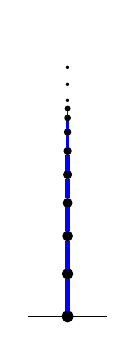
\begin{tikzpicture}
	\begin{scope} [every node/.style={scale=0.3, style=circle, draw, fill=black}]
		\node [scale=1.4] (1) at (0, -1.80){};
		\node [scale=1.3] (2) at (0, -1.26){};
		\node [scale=1.2] (3) at (0, -0.78){};
		\node [scale=1.1] (4) at (0, -0.36){};
		\node [scale=1]   (5) at (0, 0)      {};
		\node [scale=0.9] (6) at (0, 0.3)  {};
		\node [scale=0.8] (7) at (0, 0.54) {};
		\node [scale=0.7] (8) at (0, 0.72) {};
		\node [scale=0.6] (9) at (0, 0.84) {};
		\node [scale=0.2, fill=white, draw=none] at (0, 1.1) {$\vdots$};
	\end{scope}
	\draw (-0.5,-1.80) -- (0.5, -1.80);
	\draw[blue, ultra thick] (1)--(2);
	\draw[blue, ultra thick] (2)--(3);
	\draw[blue, ultra thick] (3)--(4);
	\draw[blue, ultra thick] (4)--(5);
	\draw[blue, ultra thick] (5)--(6);
	\draw[blue, thick] (6)--(7);
	\draw[blue, thick] (7)--(8);
	\draw[blue] (8)--(9);
	\node[scale=1.5] at (0, 1.3) {\scriptsize$\vdots$};
\end{tikzpicture}
\end{center}
\end{figure}

In the game above, left has an infinite number of possible moves, but \todo{his/her} move always leads to an integer. What is the value of this game? $G = \{\mathbb{N} | \}$, the number ``the largest integer plus one". It happens that this number has been baptized much earlier in mathematics of $\omega$.













